% Copyright 2004 by Till Tantau <tantau@users.sourceforge.net>.
%
% In principle, this file can be redistributed and/or modified under
% the terms of the GNU Public License, version 2.
%
% However, this file is supposed to be a template to be modified
% for your own needs. For this reason, if you use this file as a
% template and not specifically distribute it as part of a another
% package/program, I grant the extra permission to freely copy and
% modify this file as you see fit and even to delete this copyright
% notice. 

\documentclass{beamer}

% There are many different themes available for Beamer. A comprehensive
% list with examples is given here:
% http://deic.uab.es/~iblanes/beamer_gallery/index_by_theme.html
% You can uncomment the themes below if you would like to use a different
% one:
%\usetheme{AnnArbor}
%\usetheme{Antibes}
%\usetheme{Bergen}
%\usetheme{Berkeley}
%\usetheme{Berlin}
%\usetheme{Boadilla}
%\usetheme{boxes}
\usetheme{CambridgeUS}
%\usetheme{Copenhagen}
%\usetheme{Darmstadt}
%\usetheme{default}
%\usetheme{Frankfurt}
%\usetheme{Goettingen}
%\usetheme{Hannover}
%\usetheme{Ilmenau}
%\usetheme{JuanLesPins}
%\usetheme{Luebeck}
%\usetheme{Madrid}
%\usetheme{Malmoe}
%\usetheme{Marburg}
%\usetheme{Montpellier}
%\usetheme{PaloAlto}
%\usetheme{Pittsburgh}
%\usetheme{Rochester}
%\usetheme{Singapore}
%\usetheme{Szeged}
%\usetheme{Warsaw}

\usepackage[USenglish]{babel}
\usepackage[latin1]{inputenc}
\usepackage{booktabs}
\usepackage[scale=2]{ccicons}
\usepackage{pgfplots}
\usepackage{xspace}
\usepackage{enumerate}
\usepackage{amsthm}
%\usepackage[alf]{abntex2cite}
%\usepackage{subcaption}
%\usepgfplotslibrary{dateplot}
\usepackage{graphicx}
\usepackage{mathtools}
%\DeclarePairedDelimiter\abs{\lvert}{\rvert}%
%\usepackage{latexsym}
%\usepackage{amsmath}
%\usepackage[T1]{fontenc}
%\usepackage{fetamont}
%\usepackage{mathrsfs}
\usepackage{subfigure}
%\usepackage{chngcntr}
%\usepackage{fancyhdr}
%\usepackage{xmpmulti}
%\usepackage{animate}
\usepackage{ragged2e}
\usepackage{pdfpages}
\usepackage{epstopdf}

\setbeamertemplate{caption}[numbered]
%\setbeamertemplate{footline}[]{}
\setbeamertemplate{navigation symbols}{}
\setbeamertemplate{caption}{\raggedright\insertcaption\par}

\setbeamertemplate{enumerate items}[default]


\makeatletter
\define@key{beamerframe}{standout}[true]{%
	\setbeamertemplate{footline}{}%
}
\makeatother

%\setbeamertemplate{footline}
%{
%	\leavevmode%
%	\hbox{%
%		\begin{beamercolorbox}[wd=.3\paperwidth,ht=2.25ex,dp=1ex,center]{author in head/foot}%
%			\usebeamerfont{author in head/foot}\insertshortauthor
%		\end{beamercolorbox}%
%		\begin{beamercolorbox}[wd=.4\paperwidth,ht=2.25ex,dp=1ex,center]{title in center/foot}%
%			\usebeamerfont{title in head/foot}\insertshorttitle\hspace*{3em}
%		\end{beamercolorbox}%
%		\begin{beamercolorbox}[wd=.3\paperwidth,ht=2.25ex,dp=1ex,center]{conf and page/foot}%
%			\usebeamerfont{conf and page/foot}\insertshortdate\hspace*{3em}
%			\insertframenumber{} / \inserttotalframenumber\hspace*{1ex}
%		\end{beamercolorbox}}%
%	\vskip0pt%
%%}
%\setbeamercolor{title}{fg=red!70!black}
%\setbeamercolor{subtitle}{fg=black!100}
%\setbeamercolor{author}{fg=blue!50!black}
%\setbeamercolor{institute}{fg=blue!70!black}
%\setbeamercolor{frametitle}{fg=red!90!black}
%\setbeamercolor{framesubtitle}{fg=red!80!green!50}
\addtocounter{framenumber}{-1}
\titlegraphic{
	\vspace{\fill}
	
\includegraphics[width = 1.5cm]{template/ufmg-logo.png}
	 \hspace*{\fill}
	
\includegraphics[height=0.8cm]{template/macsin-logo.pdf}
}

\title[Defesa de Mestrado]{Sensor Fusion for Irregularly Sampled Systems}

% A subtitle is optional and this may be deleted
%\subtitle{Optional Subtitle}

\author{Taiguara Tupinamb�s}
% - Give the names in the same order as the appear in the paper.
% - Use the \inst{?} command only if the authors have different
%   affiliation.

\institute[]{Laborat�rio de Modelagem, An�lise e Controle de Sistemas N�o-Lineares (MACSIN) \\ Programa de P�s-Gradua��o em Engenharia El�trica (PPGEE) \\ Universidade Federal de Minas Gerais (UFMG)}

\vspace{0.5cm}

\date[Fevereiro 2019]{21 de Fevereiro, 2019}
% - Either use conference name or its abbreviation.
% - Not really informative to the audience, more for people (including
%   yourself) who are reading the slides online



\subject{Electrical Engineering}
% This is only inserted into the PDF information catalog. Can be left
% out. 

% If you have a file called "university-logo-filename.xxx", where xxx
% is a graphic format that can be processed by latex or pdflatex,
% resp., then you can add a logo as follows:

% \pgfdeclareimage[height=0.5cm]{university-logo}{university-logo-filename}
% \logo{\pgfuseimage{university-logo}}

% Delete this, if you do not want the table of contents to pop up at
% the beginning of each subsection:
\AtBeginSubsection[]
{\addtocounter{framenumber}{-1}
\begin{frame}{Sum�rio}
	\tableofcontents[currentsection,currentsubsection]
\end{frame}
}

% Let's get started
\begin{document}

{
\setbeamertemplate{footline}{} 
	\begin{frame}
	\titlepage
\end{frame}
}
\addtocounter{framenumber}{-1}
%
%\begin{frame}
%  \titlepage
%\end{frame}

\begin{frame}{Sum�rio}
\tableofcontents
% You might wish to add the option [pausesections]
\end{frame}

% Section and subsections will appear in the presentation overview
% and table of contents.

%------------------------------------------------SECTION---------------------------------
\section{Motiva��o} 
%------------------------------------------------SUBSECTION------------------------------

\subsection{Populariza��o de Redes de Sensores}

\begin{frame}
\frametitle{Crescimento do Mercado Global de Sensores}

\begin{itemize}
	\item CAGR de 11.3\% a.a. no per�odo 2016-2022 
	\item USD 241 bilh�es em 2022
\end{itemize}
\vfill
\centering
%\caption{}t
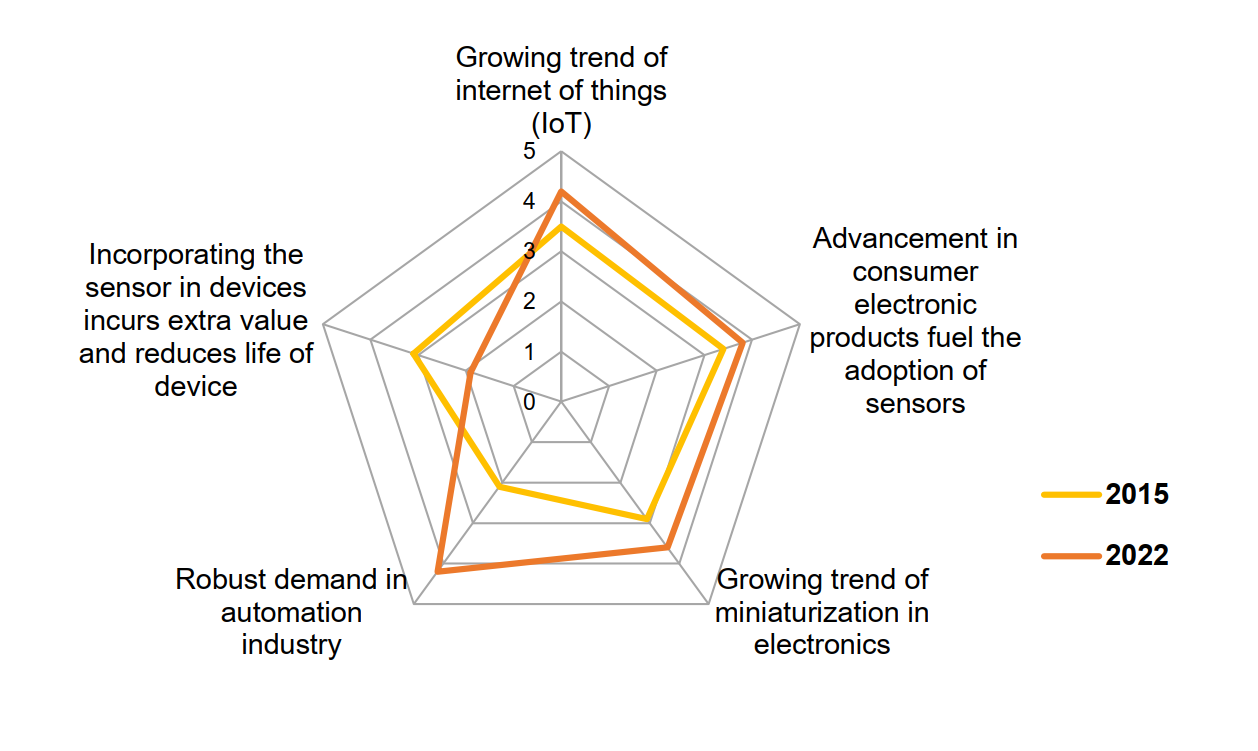
\includegraphics[width=0.6\textwidth]{images/impact_factors.png}
\par
\tiny Fonte: Allied Market Research

\end{frame}


%------------------------------------------------

\begin{frame}
\frametitle{Tend�ncias}


\begin{minipage}[t]{0.48\linewidth}
	\centering
	Internet das Coisas
	\par
	\vspace{0.5cm}
	\centering
	%\caption{}t
	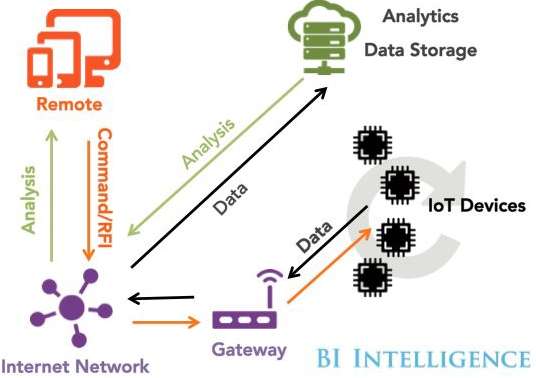
\includegraphics[width=0.8\textwidth]{images/IoT.png}
	\vspace{0.4cm}
	\par
	\tiny Fonte: Business Insider
\end{minipage}\hfill
\begin{minipage}[t]{0.48\linewidth}
	\centering
	Redes Complexas de Sensores
	\par
	\vspace{0.5cm}
	\centering
	%\caption{}t
	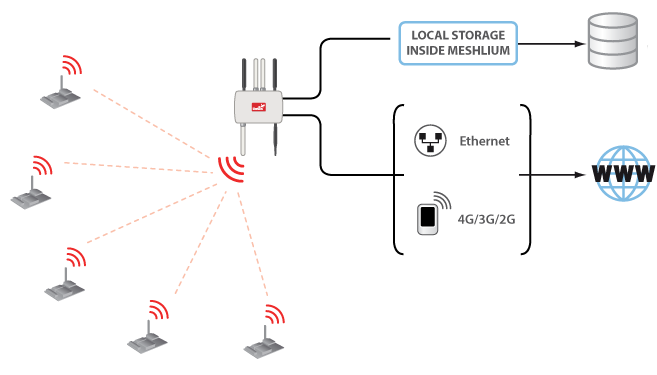
\includegraphics[width=0.85\textwidth]{images/wsn.png}
	\vspace{0.8cm}
	\par
	\tiny Fonte: Libelium
\end{minipage}

\end{frame}

%------------------------------------------------
%------------------------------------------------SUBSECTION------------------------------

\subsection{Desafios}

\begin{frame}
\frametitle{Desafios}

\begin{block}{}
	Falta de sincroniza��o entre os m�ltiplos sensores da rede pode levar a \textbf{amostragem irregular} sem informa��o confi�vel de \textbf{carimbo de tempo}
\end{block}

\vspace{1cm}

\textbf{Solu��es}:

\begin{itemize}
	\item Investir em sincroniza��o
	\item Deslocar os instantes de tempo
\end{itemize}

\end{frame}

%------------------------------------------------

\begin{frame}
\frametitle{Efeitos de se deslocar os instantes de tempo}

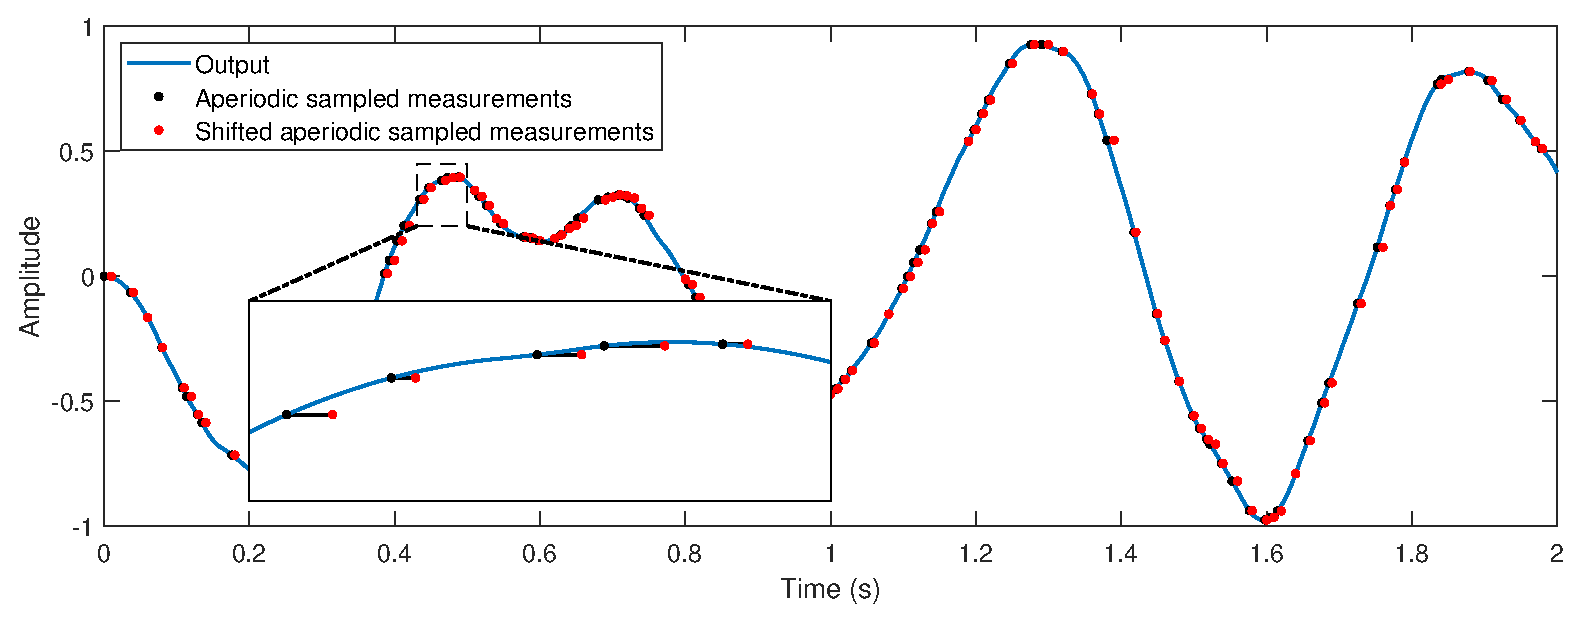
\includegraphics[width=\textwidth]{images/Gs_sampling_diff.eps}


\end{frame}

%------------------------------------------------

\begin{frame}
\frametitle{Efeitos de se deslocar os instantes de tempo}

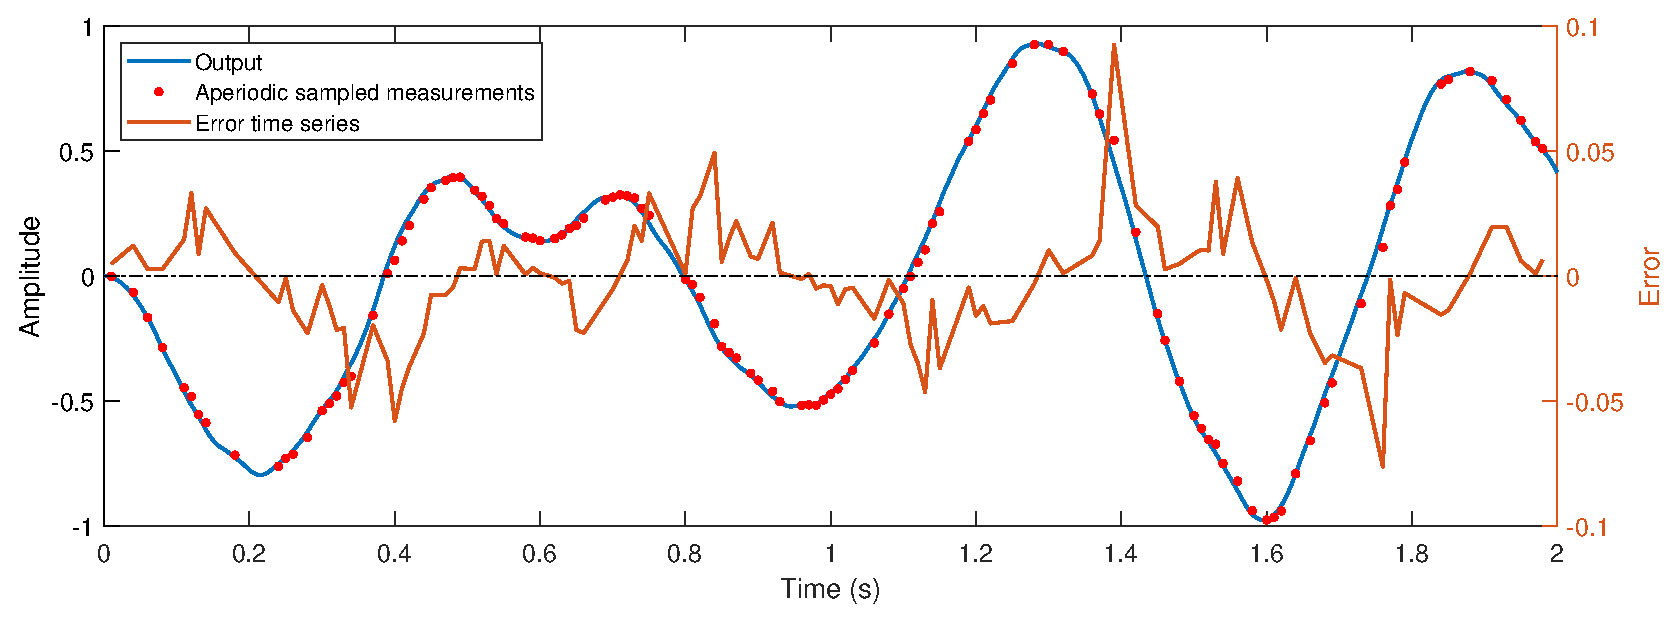
\includegraphics[width=\textwidth]{images/Gs_error.eps}


\end{frame}
%------------------------------------------------

\begin{frame}
\frametitle{Vale a pena investir em sincroniza��o?}


\begin{itemize}
	\item Qual a relev�ncia do erro para os objetivos da fus�o sensorial?
	\item Quais s�o os fatores que influenciam o desempenho?
\end{itemize}

\vfill

\begin{block}{}
\centering
Fus�o sensorial resumido ao problema de \textit{estima��o de estados}
\end{block}


\end{frame}
%------------------------------------------------
%------------------------------------------------SUBSECTION------------------------------

\subsection{Objetivos}
\begin{frame}

\frametitle{Objetivos}


\begin{enumerate}
	\item Revisar os m�todos de fus�o sensorial e o problema de amostragem irregular;
	\item Discutir os algoritmos e suas adapta��os ao modelo de medi��o amostrado irregularmente, sem carimbo de tempo;
	\item Desenvolver uma metodologia para estudar os efeitos de desconsiderar os carimbos de tempo;
	\item Aplicar a metodologia em um sistema linear e outro n�o-linear, utilizando �ndices de desempenho que avaliam a precis�o e a consist�ncia de estima��o;
\end{enumerate}

\end{frame}

%------------------------------------------------
%------------------------------------------------SUBSECTION------------------------------

\section{Metodologia}
%------------------------------------------------
\subsection{Modelo de Amostragem Irregular}
%------------------------------------------------

\begin{frame}
\frametitle{Modelo de Amostragem Irregular}

\begin{block}{}
Instantes de amostragem modelados por um processo de Poisson:
\end{block}


\begin{align}
P\left(N(t)=n\right) &= e^{-\lambda t}\frac{(\lambda t)^n}{n!} \notag\\ \notag\\
\rho_{h_k}(t) &= \lambda e^{-\lambda t}\notag
\end{align}
\end{frame}
%------------------------------------------------

\begin{frame}
\frametitle{Modelo de Amostragem Irregular}
\centering
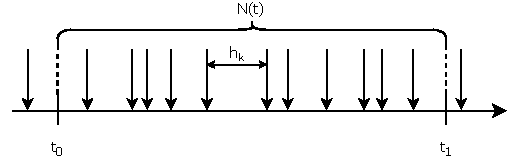
\includegraphics[width=1\textwidth]{images/poisson_proc.pdf}
\end{frame}
%------------------------------------------------


%------------------------------------------------
%
%%\section{Refer�ncias}
%\begin{frame}
%\frametitle{References}
%\bibliography{biblio}
%\end{frame}

\end{document}


